\chapter[Sensor de Rotação]{Sensor de Rotação}

\begin{enumerate}
\item \textbf{Descrição}

Segundo a Piher, evidenciado no datasheet do PST-360 \cite{sensor_rotacao}, o referente designer
renovador e único apresenta as seguintes vantagens:

\begin{itemize}
  \item Complementa os atributos do aplicativo de destino;
  \item Integridade mecânica que corresponde ao pedido do cliente pelo design.
  \item O eixo original montou o projeto que monta no ponto de pivô da aplicação;

  \item Sem alavancas , bielas ou interfaces mecânicas necessárias;

  \item Adapta-se a excentricidade do eixo, tolerâncias de montagem e
  desgaste mecânico ao longo da vida da aplicação;

\end{itemize}

\item \textbf{Especificações do Sensor PST-360}

De acordo com o Datasheet \cite{sensor_rotacao} fornecido pelo fabricante Piher, o sensor escolhido
obedece as seguintes especificações:

\begin{itemize}
  \item Linearidade : +- 1\% (0,5\% em cima do pedido );
  \item Projeto magnético simples e robusto;
  \item Faixa Angular: programável de 15º a 360º;
  \item Característica de transferência linear programável (as inclinações positivas e
  uma inclinação negativa podem ser programadas na mesma característica de transferência);

  \item Resolução angular (depende do ângulo elétrico e da velocidade rotatória):
  \item Analógico e PWM: Até 12 bits;
  \item Protocolo de Série (SPI): Até 14 bits;
  \item Diferentes opções de redundância disponíveis;
  \item Características de auto diagnostico;
  \item Vida de rotação: virtualmente ilimitado (dependendo da aplicação e montagem)
  \item Temperatura de funcionamento : de -40ºC a +125ºC;
  \item Sobre a proteção da tensão e a proteção da tensão reversa;
  \item Tensão de alimentação : 5V / 12V / 15V +- 10%
  \item Corrente de alimentação:
  \item 8.5mA para a única versão.
  \item 17mA para a versão redundante.
  \item IP67 (eletrônica);
  \item Cabeamento personalizado e configurações de conector;
\end{itemize}

\item \textbf{Exemplos de aplicações}

\begin{itemize}
  \item  Angulo de ponto do pivô que detecta para todas as aplicações;
  \item Fora da estrada/ direção da estrada;
  \item Detecção da posição de pedal;

  \item Máquinas agrícolas, braços de elevadores hidráulicos, colheres, articulações/junções;

  \item Empilhadeiras / manuseio de materiais;

  \item Bombas industriais;

  \item Robótica;

\end{itemize}


\begin{figure}[h]
  \centering
  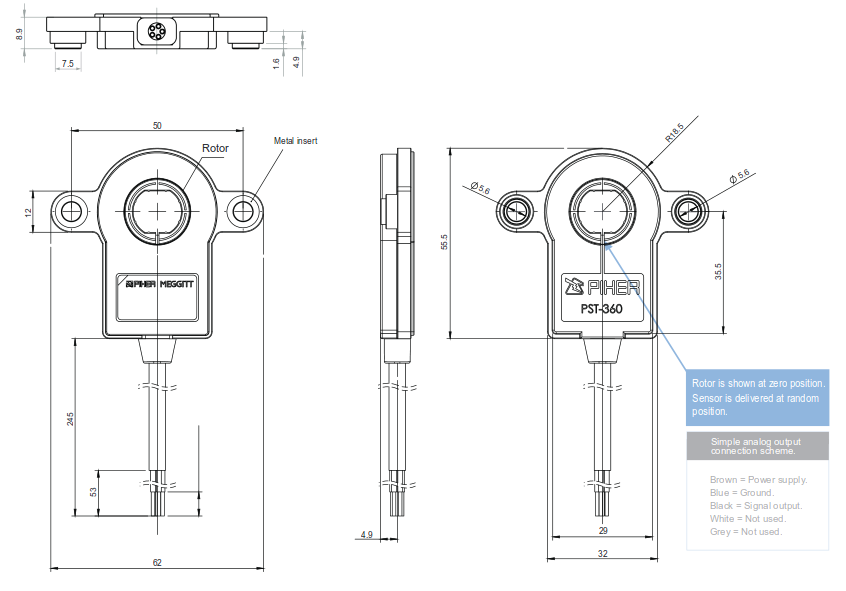
\includegraphics[width=300px, scale=1]{figuras/pst_dimensoes}
  \caption{ Dimensões do PST-360 \cite{sensor_rotacao}}
\label{fig:pst_dimensoes}
\end{figure}

\begin{figure}[h]
  \centering
  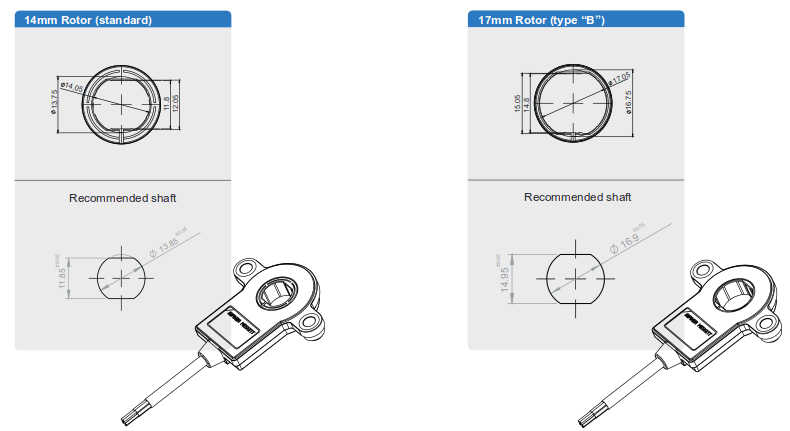
\includegraphics[width=300px, scale=1]{figuras/pst_dimensoes2}
  \caption{ Dimensões do PST-360 \cite{sensor_rotacao}}
\label{fig:pst_dimensoes2}
\end{figure}

\item \textbf{Funções de saída padrão}

\begin{figure}[h]
  \centering
  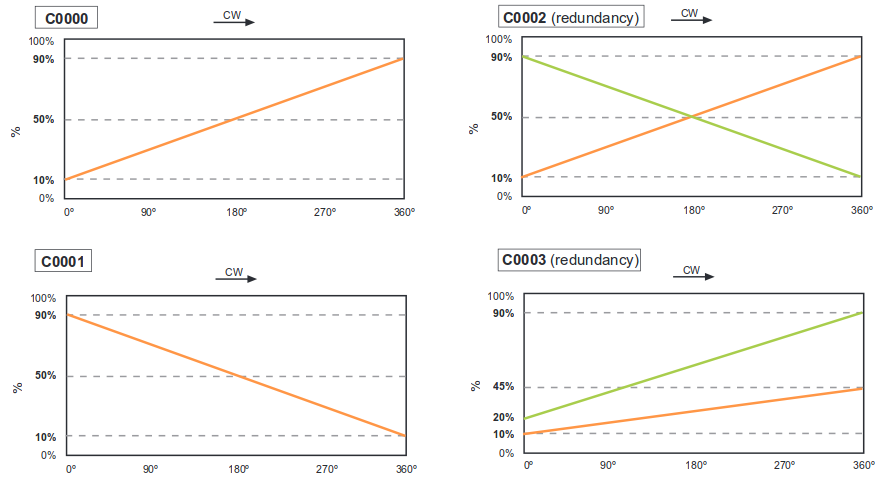
\includegraphics[width=300px, scale=1]{figuras/pst_saida_padrao}
  \caption{ Exemplos de funções padrões geradas pelo PST-360 \cite{sensor_rotacao}}
\label{fig:pst_saida_padrao}
\end{figure}

As partes ferromagnéticas perto do ambiente do sensor, incluindo o eixo,
podem modificar o desempenho do mesmo.
\end{enumerate}
